\documentclass[11pt]{article}


\usepackage{fullpage}
\usepackage{graphicx}
\usepackage{amsmath}
\usepackage{amssymb}
\usepackage{amsthm}
\usepackage{fancyvrb}

\newcommand{\myname}{Mehshan Mustafa}

\newenvironment{theorem}[2][Theorem]{\begin{trivlist}
\item[\hskip \labelsep {\bfseries #1}\hskip \labelsep {\bfseries #2.}]}{\end{trivlist}}
\newenvironment{lemma}[2][Lemma]{\begin{trivlist}
\item[\hskip \labelsep {\bfseries #1}\hskip \labelsep {\bfseries #2.}]}{\end{trivlist}}
\newenvironment{exercise}[2][Exercise]{\begin{trivlist}
\item[\hskip \labelsep {\bfseries #1}\hskip \labelsep {\bfseries #2.}]}{\end{trivlist}}
\newenvironment{problem}[2][Problem]{\begin{trivlist}
\item[\hskip \labelsep {\bfseries #1}\hskip \labelsep {\bfseries #2.}]}{\end{trivlist}}
\newenvironment{question}[2][Question]{\begin{trivlist}
\item[\hskip \labelsep {\bfseries #1}\hskip \labelsep {\bfseries #2.}]}{\end{trivlist}}
\newenvironment{corollary}[2][Corollary]{\begin{trivlist}
\item[\hskip \labelsep {\bfseries #1}\hskip \labelsep {\bfseries #2.}]}{\end{trivlist}}
\newenvironment{solution}{\begin{proof}[Solution]}{\end{proof}}
\newenvironment{idea}[2][Proof Idea.]{\textit{#1} #2}



\parindent0in
\pagestyle{plain}
\thispagestyle{plain}

\usepackage{csquotes}
\usepackage[shortlabels]{enumitem}

\newcommand{\dated}{\today}
\newcommand{\token}[1]{\langle \text{#1} \rangle}

\begin{document}

\textbf{Introduction to the Theory of
Computation}\hfill\textbf{\myname}\\[0.01in]
\textbf{Chapter 7: Time Complexity}\hfill\textbf{\dated}\\
\smallskip\hrule\bigskip

\begin{problem}{7.27}
A cut in an undirected graph is a separation of the vertices $V$ into two disjoint
subsets $S$ and $T$. The size of a cut is the number of edges that have one endpoint
in $S$ and the other in $T$. Let
\[
MAX-CUT = \{\langle G, k \rangle \ | \ G \text{ has a cut of size } k \text{ or more}\}.
\]
Show that $MAX-CUT$ is NP-complete. You may assume the result of Problem 7.26.
\end{problem}

\begin{proof}
To show that $MAX-CUT$ is NP-complete, we must show that it is in NP and that all NP-problems are polynomial time reducible to it. The first part is easy; a certificate is simply two disjoint subsets of $V$ having cut size of $k$ or more. To prove the second part, we show that $\neq$\textit{SAT} is polynomial time reducible to $MAX-CUT$. \\

The reduction converts a 3cnf-formula $\phi$ into an undirected graph $G$ and
a number $k$, so that $\phi$ has a satisfying $\neq$\textit{-assignment}, iff G has a cut of size $k$. The graph contains gadgets that mimic the variables and clauses of the formula. \\

The variable gadget for variable $x$ is a collection of $3c$ nodes labeled with $x$ and another $3c$ node labeled with $x$, where $c$ is the number of clauses. All nodes labeled $x$ are connected with all nodes labeled $x$. The clause gadget is a triangle of three edges connecting three nodes labeled with the literals appearing in the clause. Do not use the same node in more than one clause gadget. Finally, we chose k to be the maximum possible cut size of $l \times (3c)^2 + 2c$ in $G$, where $l$ is the number of variables in $\phi$.

Phi cannot have a cluase with 3 same literals.

\end{proof}

\begin{center}
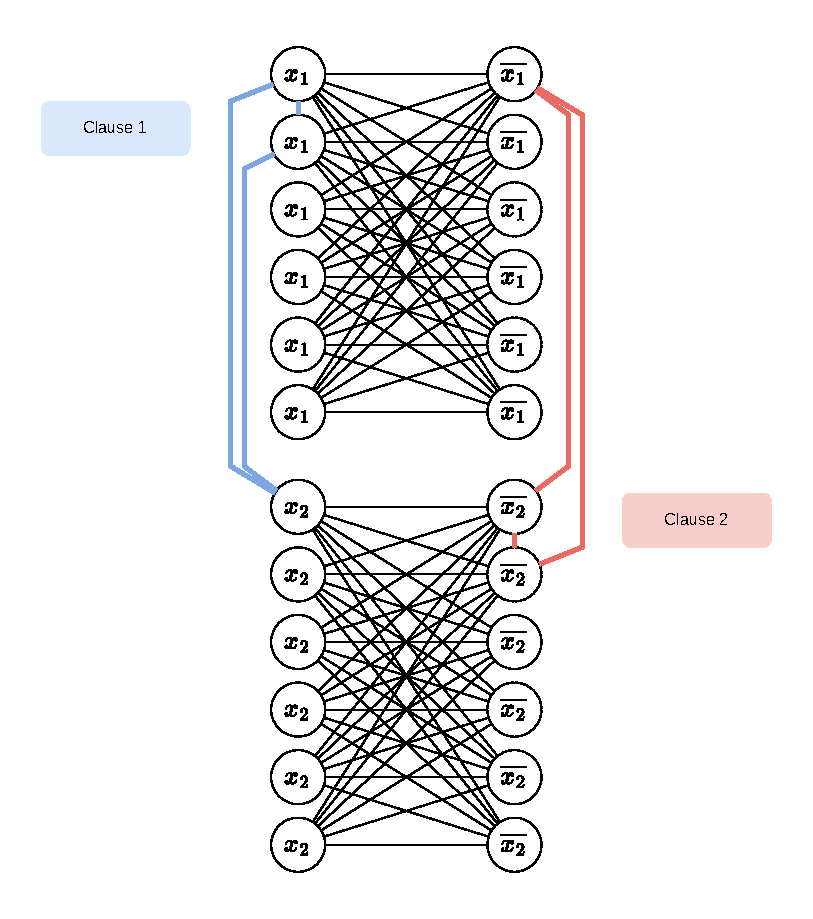
\includegraphics[scale=1.0]{Figures/Problem7.27a.pdf} \\
Graph $G$ for $\phi = (x_1 \vee x_1 \vee x_2) \wedge (\overline{x_1} \vee \overline{x_2} \vee \overline{x_2})$.
\end{center}

\end{document}